
%% This style is provided exclusively for the ICSE 2012 main conference,
%% ICSE 2012 co-located events, and ICSE 2012 workshops.

%% bare_conf_ICSE12.tex
%% V1.4
%% 2012-01-21
%%

%% This is a skeleton file demonstrating the use of IEEEtran.cls
%% (requires IEEEtran.cls version 1.7 or later) with an IEEE conference paper.
%%
%% Support sites:
%% http://www.michaelshell.org/tex/ieeetran/
%% http://www.ctan.org/tex-archive/macros/latex/contrib/IEEEtran/
%% and
%% http://www.ieee.org/

%%*************************************************************************
%% Legal Notice:
%% This code is offered as-is without any warranty either expressed or
%% implied; without even the implied warranty of MERCHANTABILITY or
%% FITNESS FOR A PARTICULAR PURPOSE! 
%% User assumes all risk.
%% In no event shall IEEE or any contributor to this code be liable for
%% any damages or losses, including, but not limited to, incidental,
%% consequential, or any other damages, resulting from the use or misuse
%% of any information contained here.
%%
%% All comments are the opinions of their respective authors and are not
%% necessarily endorsed by the IEEE.
%%
%% This work is distributed under the LaTeX Project Public License (LPPL)
%% ( http://www.latex-project.org/ ) version 1.3, and may be freely used,
%% distributed and modified. A copy of the LPPL, version 1.3, is included
%% in the base LaTeX documentation of all distributions of LaTeX released
%% 2003/12/01 or later.
%% Retain all contribution notices and credits.
%% ** Modified files should be clearly indicated as such, including  **
%% ** renaming them and changing author support contact information. **
%%
%% File list of work: IEEEtran.cls, IEEEtran_HOWTO.pdf, bare_adv.tex,
%%                    bare_conf.tex, bare_jrnl.tex, bare_jrnl_compsoc.tex
%%*************************************************************************

% *** Authors should verify (and, if needed, correct) their LaTeX system  ***
% *** with the testflow diagnostic prior to trusting their LaTeX platform ***
% *** with production work. IEEE's font choices can trigger bugs that do  ***
% *** not appear when using other class files.                            ***
% The testflow support page is at:
% http://www.michaelshell.org/tex/testflow/



% Note that the a4paper option is mainly intended so that authors in
% countries using A4 can easily print to A4 and see how their papers will
% look in print - the typesetting of the document will not typically be
% affected with changes in paper size (but the bottom and side margins will).
% Use the testflow package mentioned above to verify correct handling of
% both paper sizes by the user's LaTeX system.
%
% Also note that the "draftcls" or "draftclsnofoot", not "draft", option
% should be used if it is desired that the figures are to be displayed in
% draft mode.
%
\documentclass[10pt, conference, compsocconf]{IEEEtran}
% Add the compsocconf option for Computer Society conferences.
%
% If IEEEtran.cls has not been installed into the LaTeX system files,
% manually specify the path to it like:
% \documentclass[conference]{../sty/IEEEtran}


\usepackage{balance}


% Some very useful LaTeX packages include:
% (uncomment the ones you want to load)


% *** MISC UTILITY PACKAGES ***
%
%\usepackage{ifpdf}
% Heiko Oberdiek's ifpdf.sty is very useful if you need conditional
% compilation based on whether the output is pdf or dvi.
% usage:
% \ifpdf
%   % pdf code
% \else
%   % dvi code
% \fi
% The latest version of ifpdf.sty can be obtained from:
% http://www.ctan.org/tex-archive/macros/latex/contrib/oberdiek/
% Also, note that IEEEtran.cls V1.7 and later provides a builtin
% \ifCLASSINFOpdf conditional that works the same way.
% When switching from latex to pdflatex and vice-versa, the compiler may
% have to be run twice to clear warning/error messages.






% *** CITATION PACKAGES ***
%
\usepackage{cite}
% cite.sty was written by Donald Arseneau
% V1.6 and later of IEEEtran pre-defines the format of the cite.sty package
% \cite{} output to follow that of IEEE. Loading the cite package will
% result in citation numbers being automatically sorted and properly
% "compressed/ranged". e.g., [1], [9], [2], [7], [5], [6] without using
% cite.sty will become [1], [2], [5]--[7], [9] using cite.sty. cite.sty's
% \cite will automatically add leading space, if needed. Use cite.sty's
% noadjust option (cite.sty V3.8 and later) if you want to turn this off.
% cite.sty is already installed on most LaTeX systems. Be sure and use
% version 4.0 (2003-05-27) and later if using hyperref.sty. cite.sty does
% not currently provide for hyperlinked citations.
% The latest version can be obtained at:
% http://www.ctan.org/tex-archive/macros/latex/contrib/cite/
% The documentation is contained in the cite.sty file itself.






% *** GRAPHICS RELATED PACKAGES ***
%
\ifCLASSINFOpdf
  \usepackage[pdftex]{graphicx}
  % declare the path(s) where your graphic files are
  \graphicspath{{../pdf/}{../jpeg/}}
  % and their extensions so you won't have to specify these with
  % every instance of \includegraphics
  \DeclareGraphicsExtensions{.pdf,.jpeg,.png}
\else
  % or other class option (dvipsone, dvipdf, if not using dvips). graphicx
  % will default to the driver specified in the system graphics.cfg if no
  % driver is specified.
  \usepackage[dvips]{graphicx}
  % declare the path(s) where your graphic files are
  \graphicspath{{../eps/}}
  % and their extensions so you won't have to specify these with
  % every instance of \includegraphics
  \DeclareGraphicsExtensions{.eps}
\fi
% graphicx was written by David Carlisle and Sebastian Rahtz. It is
% required if you want graphics, photos, etc. graphicx.sty is already
% installed on most LaTeX systems. The latest version and documentation can
% be obtained at: 
% http://www.ctan.org/tex-archive/macros/latex/required/graphics/
% Another good source of documentation is "Using Imported Graphics in
% LaTeX2e" by Keith Reckdahl which can be found as epslatex.ps or
% epslatex.pdf at: http://www.ctan.org/tex-archive/info/
%
% latex, and pdflatex in dvi mode, support graphics in encapsulated
% postscript (.eps) format. pdflatex in pdf mode supports graphics
% in .pdf, .jpeg, .png and .mps (metapost) formats. Users should ensure
% that all non-photo figures use a vector format (.eps, .pdf, .mps) and
% not a bitmapped formats (.jpeg, .png). IEEE frowns on bitmapped formats
% which can result in "jaggedy"/blurry rendering of lines and letters as
% well as large increases in file sizes.
%
% You can find documentation about the pdfTeX application at:
% http://www.tug.org/applications/pdftex





% *** MATH PACKAGES ***
%
\usepackage[cmex10]{amsmath}
% A popular package from the American Mathematical Society that provides
% many useful and powerful commands for dealing with mathematics. If using
% it, be sure to load this package with the cmex10 option to ensure that
% only type 1 fonts will utilized at all point sizes. Without this option,
% it is possible that some math symbols, particularly those within
% footnotes, will be rendered in bitmap form which will result in a
% document that can not be IEEE Xplore compliant!
%
% Also, note that the amsmath package sets \interdisplaylinepenalty to 10000
% thus preventing page breaks from occurring within multiline equations. Use:
\interdisplaylinepenalty=2500
% after loading amsmath to restore such page breaks as IEEEtran.cls normally
% does. amsmath.sty is already installed on most LaTeX systems. The latest
% version and documentation can be obtained at:
% http://www.ctan.org/tex-archive/macros/latex/required/amslatex/math/





% *** SPECIALIZED LIST PACKAGES ***
%
%\usepackage{algorithmic}
% algorithmic.sty was written by Peter Williams and Rogerio Brito.
% This package provides an algorithmic environment fo describing algorithms.
% You can use the algorithmic environment in-text or within a figure
% environment to provide for a floating algorithm. Do NOT use the algorithm
% floating environment provided by algorithm.sty (by the same authors) or
% algorithm2e.sty (by Christophe Fiorio) as IEEE does not use dedicated
% algorithm float types and packages that provide these will not provide
% correct IEEE style captions. The latest version and documentation of
% algorithmic.sty can be obtained at:
% http://www.ctan.org/tex-archive/macros/latex/contrib/algorithms/
% There is also a support site at:
% http://algorithms.berlios.de/index.html
% Also of interest may be the (relatively newer and more customizable)
% algorithmicx.sty package by Szasz Janos:
% http://www.ctan.org/tex-archive/macros/latex/contrib/algorithmicx/




% *** ALIGNMENT PACKAGES ***
%
%\usepackage{array}
% Frank Mittelbach's and David Carlisle's array.sty patches and improves
% the standard LaTeX2e array and tabular environments to provide better
% appearance and additional user controls. As the default LaTeX2e table
% generation code is lacking to the point of almost being broken with
% respect to the quality of the end results, all users are strongly
% advised to use an enhanced (at the very least that provided by array.sty)
% set of table tools. array.sty is already installed on most systems. The
% latest version and documentation can be obtained at:
% http://www.ctan.org/tex-archive/macros/latex/required/tools/


\usepackage{mdwmath}
\usepackage{mdwtab}
% Also highly recommended is Mark Wooding's extremely powerful MDW tools,
% especially mdwmath.sty and mdwtab.sty which are used to format equations
% and tables, respectively. The MDWtools set is already installed on most
% LaTeX systems. The lastest version and documentation is available at:
% http://www.ctan.org/tex-archive/macros/latex/contrib/mdwtools/


% IEEEtran contains the IEEEeqnarray family of commands that can be used to
% generate multiline equations as well as matrices, tables, etc., of high
% quality.


%\usepackage{eqparbox}
% Also of notable interest is Scott Pakin's eqparbox package for creating
% (automatically sized) equal width boxes - aka "natural width parboxes".
% Available at:
% http://www.ctan.org/tex-archive/macros/latex/contrib/eqparbox/





% *** SUBFIGURE PACKAGES ***
\usepackage[tight,footnotesize]{subfigure}
% subfigure.sty was written by Steven Douglas Cochran. This package makes it
% easy to put subfigures in your figures. e.g., "Figure 1a and 1b". For IEEE
% work, it is a good idea to load it with the tight package option to reduce
% the amount of white space around the subfigures. subfigure.sty is already
% installed on most LaTeX systems. The latest version and documentation can
% be obtained at:
% http://www.ctan.org/tex-archive/obsolete/macros/latex/contrib/subfigure/
% subfigure.sty has been superceeded by subfig.sty.



%\usepackage[caption=false]{caption}
%\usepackage[font=footnotesize]{subfig}
% subfig.sty, also written by Steven Douglas Cochran, is the modern
% replacement for subfigure.sty. However, subfig.sty requires and
% automatically loads Axel Sommerfeldt's caption.sty which will override
% IEEEtran.cls handling of captions and this will result in nonIEEE style
% figure/table captions. To prevent this problem, be sure and preload
% caption.sty with its "caption=false" package option. This is will preserve
% IEEEtran.cls handing of captions. Version 1.3 (2005/06/28) and later 
% (recommended due to many improvements over 1.2) of subfig.sty supports
% the caption=false option directly:
%\usepackage[caption=false,font=footnotesize]{subfig}
%
% The latest version and documentation can be obtained at:
% http://www.ctan.org/tex-archive/macros/latex/contrib/subfig/
% The latest version and documentation of caption.sty can be obtained at:
% http://www.ctan.org/tex-archive/macros/latex/contrib/caption/




% *** FLOAT PACKAGES ***
%
%\usepackage{fixltx2e}
% fixltx2e, the successor to the earlier fix2col.sty, was written by
% Frank Mittelbach and David Carlisle. This package corrects a few problems
% in the LaTeX2e kernel, the most notable of which is that in current
% LaTeX2e releases, the ordering of single and double column floats is not
% guaranteed to be preserved. Thus, an unpatched LaTeX2e can allow a
% single column figure to be placed prior to an earlier double column
% figure. The latest version and documentation can be found at:
% http://www.ctan.org/tex-archive/macros/latex/base/



%\usepackage{stfloats}
% stfloats.sty was written by Sigitas Tolusis. This package gives LaTeX2e
% the ability to do double column floats at the bottom of the page as well
% as the top. (e.g., "\begin{figure*}[!b]" is not normally possible in
% LaTeX2e). It also provides a command:
%\fnbelowfloat
% to enable the placement of footnotes below bottom floats (the standard
% LaTeX2e kernel puts them above bottom floats). This is an invasive package
% which rewrites many portions of the LaTeX2e float routines. It may not work
% with other packages that modify the LaTeX2e float routines. The latest
% version and documentation can be obtained at:
% http://www.ctan.org/tex-archive/macros/latex/contrib/sttools/
% Documentation is contained in the stfloats.sty comments as well as in the
% presfull.pdf file. Do not use the stfloats baselinefloat ability as IEEE
% does not allow \baselineskip to stretch. Authors submitting work to the
% IEEE should note that IEEE rarely uses double column equations and
% that authors should try to avoid such use. Do not be tempted to use the
% cuted.sty or midfloat.sty packages (also by Sigitas Tolusis) as IEEE does
% not format its papers in such ways.





% *** PDF, URL AND HYPERLINK PACKAGES ***
%
%\usepackage{url}
% url.sty was written by Donald Arseneau. It provides better support for
% handling and breaking URLs. url.sty is already installed on most LaTeX
% systems. The latest version can be obtained at:
% http://www.ctan.org/tex-archive/macros/latex/contrib/misc/
% Read the url.sty source comments for usage information. Basically,
% \url{my_url_here}.

%% Package to linebreak URLs in a sane manner.
\usepackage{url}
%% Define a new 'smallurl' style for the package that will use a smaller font.
\makeatletter
\def\url@smallurlstyle{%
  \@ifundefined{selectfont}{\def\UrlFont{\sf}}{\def\UrlFont{\small\ttfamily}}}
\makeatother
%% Now actually use the newly defined style.
\urlstyle{smallurl}
%% Define 'tinyurl' style for even smaller URLs (such as in tables)
\makeatletter
\def\url@tinyurlstyle{%
  \@ifundefined{selectfont}{\def\UrlFont{\sf}}{\def\UrlFont{\scriptsize\ttfamily}}}
\makeatother



% *** Do not adjust lengths that control margins, column widths, etc. ***
% *** Do not use packages that alter fonts (such as pslatex).         ***
% There should be no need to do such things with IEEEtran.cls V1.6 and later.
% (Unless specifically asked to do so by the journal or conference you plan
% to submit to, of course. )


% correct bad hyphenation here
\hyphenation{op-tical net-works semi-conduc-tor}


\begin{document}
%
% paper title
% can use linebreaks \\ within to get better formatting as desired
\title{Recognizing recurrent development behaviours\\ corresponding to Android OS release life-cycle}


% author names and affiliations
% use a multiple column layout for up to two different
% affiliations

\author{\IEEEauthorblockN{Pavel Senin}
\IEEEauthorblockA{CSDL laboratory, ICS Department \\University of Hawaii at Manoa\\
Honolulu, Hawaii \\ senin@hawaii.edu}
%\and
%\IEEEauthorblockN{Authors Name/s per 2nd Affiliation}
%\IEEEauthorblockA{line 1 (of Affiliation): dept. of organization (optional)\\
%line 2: name of organization (acronyms acceptable)\\
%line 3: City, Country\\
%line 4: name@xyz.com (optional)}
}

% conference papers do not typically use \thanks and this command
% is locked out in conference mode. If really needed, such as for
% the acknowledgment of grants, issue a \IEEEoverridecommandlockouts
% after \documentclass

% for over three affiliations, or if they all won't fit within the width
% of the page, use this alternative format:
% 
%\author{\IEEEauthorblockN{Michael Shell\IEEEauthorrefmark{1},
%Homer Simpson\IEEEauthorrefmark{2},
%James Kirk\IEEEauthorrefmark{3}, 
%Montgomery Scott\IEEEauthorrefmark{3} and
%Eldon Tyrell\IEEEauthorrefmark{4}}
%\IEEEauthorblockA{\IEEEauthorrefmark{1}School of Electrical and Computer Engineering\\
%Georgia Institute of Technology,
%Atlanta, Georgia 30332--0250\\ Email: see http://www.michaelshell.org/contact.html}
%\IEEEauthorblockA{\IEEEauthorrefmark{2}Twentieth Century Fox, Springfield, USA\\
%Email: homer@thesimpsons.com}
%\IEEEauthorblockA{\IEEEauthorrefmark{3}Starfleet Academy, San Francisco, California 96678-2391\\
%Telephone: (800) 555--1212, Fax: (888) 555--1212}
%\IEEEauthorblockA{\IEEEauthorrefmark{4}Tyrell Inc., 123 Replicant Street, Los Angeles, California 90210--4321}}




% use for special paper notices
%\IEEEspecialpapernotice{(Invited Paper)}




% make the title area
\maketitle


\begin{abstract}
Android OS is an open-source Linux-based operating system for mobile devices developed by 
Open Handset Alliance led by Google, its SCM log was selected as a research subject for 
2012 MSR Challenge.
I attempted to apply a novel data mining technique based on SAX approximation and indexing 
of time-series with TF$\ast$ IDF weights in order to discover recurrent behaviors within 
the Android OS development process. 

By mining software process artifact trails corresponding to OMAP kernel development 
I was able to discover recurrent behaviors in the new code lines dynamics before and after
release. By building a classifier upon these behaviors I was able to succesfully recognize 
pre- and post-release behaviors within the same and similar sub-projects of Android OS.
\end{abstract}

\begin{IEEEkeywords}
Behaviors Detection, Empirical Study, Source Control System

\end{IEEEkeywords}


% For peer review papers, you can put extra information on the cover
% page as needed:
% \ifCLASSOPTIONpeerreview
% \begin{center} \bfseries EDICS Category: 3-BBND \end{center}
% \fi
%
% For peerreview papers, this IEEEtran command inserts a page break and
% creates the second title. It will be ignored for other modes.
\IEEEpeerreviewmaketitle



\section{Introduction}
% no \IEEEPARstart
As many other large open-source projects, Android OS was in the development for many years. 
Android is ``an open-source software stack for mobile phones and other devices'',
\url{http://source.android.com/} which is based on the Linux 2.6 monolithic kernel.
Development of Android begun by Android Inc., the small startup company.
In 2005 company was acquired by Google which formed the Open Handset Alliance - a consortium of 84 companies 
which announced the availability of the Android Software Development Kit (SDK) 
in November 2007. The Android OS code is open and released under the Apache License.

Git is used as a version control system for Android and source code organized into more than 
two hundreds of sub-projects. These organized by the function (kernel, UI, mailing system, etc.) and underlying hardware 
(CPU type, bluetooth communication chip, etc.). 
There are about two millions of change records registered in the Android SCM by more than 
eleven thousands of contributors within an eight years span.

By the large body of previous reserach it is shown that the change metadata is a rich 
source of software process and developers social characteristics. The ability of 
discivering of recurrent behaviors with Fourier Analysis of change events 
explained in \cite{citeulike:10377345} whether other work, such as \cite{citeulike:10392277}
relates activity time intervals and software product quality. Thus, potentially,
there is a possibility to relate the recurrent behaviors to the software product 
quality and to the software process efficiency. The first necessery part of a toolkit
aiding such a research is an efficient mechanism of dicovering recurrent behaviors
modulated by social and project-related constraints. In this paper I extend the 
previous research by introducing a universal framework for the temporal 
partitioning of software change artifacts, the data complexity reduction 
and for recurrent behaviors discovery.

\section{Contribution}
To the best of my knowledge, this work is the first attempt to study the applicability
of symbolic aggregate approximation and term frequency\textendash document frequency
weight statistics to the mining of software process artifacts trails. 
This methodology has a number of advantages. First of all, SAX facilitates significant 
reduction of the large complexity (dimensionality and noise) of temporal artifacts 
and opens the door to application of a phetora of strings and text-mining algorithms.
In turn, the TF$\ast$IDF statistics provides an efficient mechanism for 
discrimination of the signal by ranking text data. While the third component I have 
used - the relational database facilitates the efficient data slicing, indexing
and its instant retrieval.

As an example of a possible data-mining workflow demonstrating the resolving power 
and correctness of the approach I present a case study of building a classifier
for pre- and post-release recurrent behaviors. 
Whereas this classifier demonstrates a good performance within the project it was 
trained on with less than 20\% of missclassification, it has less than 15\% 
missclassification rate in similar Android OS kernel sub-projects.

\section{Motivation}
Software development is a human activity resulting in software product. The 
amount of time and effort needed to complete a software project and the 
quality of the final product are shown to be derivatives of the software
process. Thus, studying software processes is one of the important areas of
software engineering. 

Previously it was found that software development, as many other human activities,
could be successfully partitioned by the time of the day reflecting our lifestyle and habits
\cite{citeulike:10396459} \cite{citeulike:10392305}. However external constraints, 
such as employment and management constraints \cite{citeulike:6095797}, 
software release cycle, \cite{citeulike:2739216} and other, found to be able 
to significantly alter natural activity patterns. Furthermore, within open-source 
projects with diverse development community scattered over the globe and 
often following undocumented development process, the natural human activity cycles 
are often discarded as well as the development and release cycles are significantly altered.
Thus, the only feasible way to discover an open-source software process is to analyze 
its artifacts trails such as SCM logs, bug and issue tracking systems and 
mailing lists archives. Essentially these trails are event-series where every 
time-stamped event has an attached set of metadata. 
However the complexity of this data and the precision of the process 
recall impose a great challenge for the researchers.

These challenges are not new to the data-mining community and an enormous wealth 
of methods, algorithms and data structures exist helping to overcome these issues.
While some of these approaches were already implemented within the MSR framework 
such as finding of trends, periodicity and recurrent behaviors through the linear 
predictive coding and cepstrum coefficients \cite{citeulike:3378725}, 
Fourier Transform \cite{citeulike:10377345} and coding \cite{citeulike:10377366},
many are yet to be tried.

In this paper, I investigate the application of 
Symbolic Aggregate Approximation \cite{citeulike:2821475} and the TF$\ast$IDF 
statistics \cite{citeulike:3056638} to the problem of discovering recurrent 
behaviors from software process artifacts with application to Android SCM data.

\section{Research question}
In this exploratory work I am investigating the applicability of Lin\&Keogh \cite{citeulike:2821475} 
symbolic approximation technique to the discovery of recurrent behaviors from SCM trails 
of Android OS.
The research questions I am trying to resolving are: 
\begin{itemize}
 \item Which kinds of SCM data need to be collected for such analyzes?
 \item What is the optimal way of data representation and a data storage configuration?
 \item Which partitioning (slicing) is appropriate and which set of parameters one should use for SAX approximation?
 \item Which distance metrics serves best for measuring similarity and dissimilarity?
 \item What is the general mining workflow, and which parameters are crucial for result?
\end{itemize}

\section{Experimental setup and methods}
\subsection{Data collection and organization}
Two XML files were offered for the MSR challenge. These contain the most of the information obtainable 
from Google-hosted git source code repository as well as from bug and issue tracking system.
While the issues and comment XML file contains nearly all information available in repository, 
the change XML provided for this challenge contains only a fraction of all of the information.

The thirteen data fields of the change trail XML file provide information about the revision 
tree, author and a committer identification, change message and affected targets. 
Since I am focusing on the mining of temporal patterns for inferring recurrent behaviors, 
in addition to the existing data I have collected many auxiliary data about change. By creating
a local mirror and by iterating over existing commit hashes I was able to recover the auxiliary 
data for 68\% of existing commits. The rest 32\% of change information is unretrievable and 
belongs to legacy projects or is lost and unrecoverable due to the changes in Android repository. 

For every recoverable change record I collected a summary of added, modified and deleted files 
as well as a summary about LOC changes: added, modified or deleted lines. All this information 
was stored in the database backend. Main tables of this database correspond to change 
and issue events; these accompanied with change target table, issue, comments and 
tables for contributors. Overall, the database was normalized and optimized for the fast 
retrieval of change and issue information using SQL language.

\subsection{Temporal data partitioning}
Following the previous research \cite{citeulike:10392277}, I have partitioned the 
change trails by the time of the day using time windows of
\begin{itemize}
 \item Full day, 12AM - 12AM
    \item Late night, 12AM - 04AM  
    \item Early morning, 04AM - 08AM  
    \item Day, 08AM - 05PM  
    \item Night, 05PM - 12AM
\end{itemize}
then aggregated within these windows values for commits, added/edited/deleted 
lines and targets. By having such a table it takes a fractions of a second to retrieve 
a summary of early morning added lines for January 2007 for a particular sub-project and
a group of contributors having emails with a domain ``...@ibm.com''.

\subsection{Symbolic approximation and indexing}
SAX algorithm requires three parameters where the first is the sliding window size, 
second is the PAA approximation size and the third parameter is the SAX Alphabet size.

In this work I have selected three sizes for sliding window: 7 days, 14 days and 30 days as 
these represent an intuitive and logical intervals of a week, two weeks and a month. 
For the PAA reduction I choose 4 steps for 7 days window, 6 steps for a bi-weekly interval,
and 10 steps for a monthly window.
Finally the alphabet, I choose 3 letters for weekly window, and 5 letters for bi-weekly and monthly windows.

By applying SAX to the pre-aggregated data I have obtained their symbolic temporal 
representation. Do I need a figure explaining SAX transform here?

%\begin{table}
%  \caption{Sliding window, PAA and alphabet size choices.}
%  \centering
%  \label{tab:parameters}
%  \begin{tabular}{ | l | c | c |}
%  \hline                       
%  Sliding window size & PAA size & Alphabet size \\
%  \hline 
%    one week (7 days) & 4 & 3 \\  
%    two weeks (14 days) & 6 & 5 \\ 
%    month (30 days) & 10 & 5 \\ 
%  \hline  
%  \end{tabular}
%\end{table}

\subsection{Token-based distance metrics}
For the experiments I have selected three similarity metrics. 
First one is based on the SAX min distance and the Euclidean distance which applied to vector of tokens 
sorted by frequency observed in the aggregated symbolic stream corresponding to selected stream class,
aggregation parameters, user, project and time-interval of the interest. 
\begin{equation}
D(S,T) = \sqrt{ \sum SAXdist(s_{i},t_{i})^{2} }
\end{equation} 
where $SAXdist$ is the the SAX distance based on the Normal alphabet.

As an alternative I have tried the Jaccard similarity between two sets $S$ and $T$ which is simply 
\begin{equation}
J_{\delta}(S,T) = \frac{|S\cup T| - |S\cap T|}{|S\cup T|}
\end{equation} 
and the $TF\ast IDF$ similarity or which defined as a dot product 
\begin{equation}
 TFIDF(S,T) = \sum_{\omega \in S \cap T} V(\omega, S) \cdot V(\omega, T)
\end{equation} 
where 
\begin{equation}
 V(\omega, S) = \frac { V^{\prime} (\omega,S) } { \sqrt{ \sum_{\omega^{\prime}} V^{\prime} (\omega,S)^{2}} }
\end{equation} 
is a normalization of $TF\ast IDF$ (product of token frequency and inverse document frequency):
\begin{equation}
 V^{\prime} (\omega,S) = \log(TF_{\omega, S} +1) \cdot \log(IDF_{\omega})
\end{equation} 
where $IDF_{\omega}$ is a measure of the general importance of the pattern among all users
\begin{equation}
 IDF_{\omega} = \frac{|D|}{DF(\omega)}
\end{equation} 
where $|D|$ is cardinality of $D$ - the total number of users, and $DF(\omega)$ is the number of users having $\omega$ pattern in their activity set.
%% See \href{http://en.wikipedia.org/wiki/TFIDF}

\section{Clustering}
While the application of the SAX distance and Jaccard similarity yields a single number allowing
the use of the convenient clustering libraries such as $hclust()$ and $kmeans()$ of R for manipulation
with sparse vectors produced by the $TF\ast IDF$ application I used $sparcl()$ R package for hierarchical
clustering and my own implementation of $k-means$ clustering.

\begin{table*}
  \caption{Pre- and post-release patterns, their $TF\ast IDF$ weights and sample curves.}
  \label{tab:tokens}
  \begin{tabular}{ | b{1.5cm} | c | c | c | c | c | c | c | c | c | c | c |}
  \hline
release & "bbac" & "abca" & "babc" & "bbba" & "bcaa" & "bcbb" & "ccaa" & "cbaa" & "bbcb" & "bbbb" & "bbbc"\\ 
  \hline
 post-2.0 & 0.63 & 0 & 0.63 & 0 & 0 & 0 & 0 & 0.39 & 0.24 & 0.06 & 0\\ 
 post-1.0 & 0 & 0.93 & 0 & 0 & 0 & 0 & 0 & 0 & 0 & 0.09 & 0.36\\ 
 post-1.5 & 0 & 0 & 0 & 0 & 0 & 0 & 0 & 0 & 0.79 & 0.61 & 0\\ 
 pre-1.5 & 0 & 0 & 0 & 0.23 & 0.23 & 0.91 & 0 & 0.14 & 0.18 & 0 & 0.09\\ 
 pre-2.0 & 0 & 0 & 0 & 0 & 0 & 0 & 0 & 0 & 0 & 1 & 0\\ 
 pre-2.0 & 0 & 0 & 0 & 0 & 0 & 0 & 0.79 & 0 & 0 & 0.08 & 0.61\\
 \hline 
 &  &  &  &  &  &  & &  &  &  & \\
 Sample curves corresponding to patterns &
 \includegraphics[scale=0.08]{figures/bbac.ps} &
 \includegraphics[scale=0.08]{figures/abca.ps} &  
 \includegraphics[scale=0.08]{figures/babc.ps} &  
 \includegraphics[scale=0.08]{figures/bbba.ps} &  
 \includegraphics[scale=0.08]{figures/bcaa.ps} &  
 \includegraphics[scale=0.08]{figures/bcbb.ps} &  
 \includegraphics[scale=0.08]{figures/ccaa.ps} &  
 \includegraphics[scale=0.08]{figures/cbaa.ps} &  
 \includegraphics[scale=0.08]{figures/bbcb.ps} &  
 \includegraphics[scale=0.08]{figures/bbbb.ps} &  
 \includegraphics[scale=0.08]{figures/bbbc.ps} \\
  \hline
  \end{tabular}
\end{table*}

\section{Results}
\subsection{Kernel-OMAP life cycle patterns discovery}
I arbitrary selected the Android kernel-OMAP as one of the large Android OS sub-projects. 
OMAP is a proprietary system on chips (SoCs) for portable and mobile multimedia applications 
based on general-purpose ARM architecture processor provided by Texas Instruments.

As a training set for building dictionaries of pre and post-release patterns I choose three Android releases:
\textit{Android 1.0}, \textit{Android 1.5} and \textit{Android 2.0}. For each release in the set I selected four 
weeks before the release as \textit{pre-release} and four weeks after release as \textit{post-release} 
training intervals. As an additional constraint for this experiment I have selected contributors affiliated
with $@android.com$ e-mail domain and a telemetry stream of $added\_lines$.
After pre-generated patterns retrieval with SQL query I applied hierarchical clustering 
based on $TF\ast IDF$ similarity as a sanity test. The almost perfect clustering picture \ref{fig:kernel_cluster}
indicates that there are significant differences in the pre-release and post-release weekly behaviors among 
selected contributors.

While hierarchical clustering is a good sanity test for the separation of data, the performance of K-means 
clustering is the most valuable metrics \cite{citeulike:3562}. I performed k-means on the symbolic 
representation of data using $TF\ast IDF$ statistics and the Euclidean distance. Algorithm converged after two
iterations separating pre- and post-release dictionaries with a single mismatch for the Android 2.0 pre-release.

\begin{figure}[htb]
  \centering
  \includegraphics[width=0.5\textwidth]{figures/omap-hclust.eps}
  \caption{Hierarchical clustering of pre- and post- commit patterns.}
  \label{fig:kernel_cluster}
\end{figure}

By using centroids of resulting clusters as a basis for pre and post-release patterns I tested 
the classifier on the rest of Android releases for which kernel-OMAP remained an active project
(some of the pre- and post- release interval contained non or only trivial patterns making them
ineligible for classification). This classifier was able to successfully classify more than 81\% 
of pre- and post-release behaviors (Table \ref{tab:success}).

\begin{table}
  \caption{Pre- and post-release development patterns classification results for kernel-OMAP.}
  \label{tab:success}
  \begin{tabular}{ | l | c | c c | l | c |}
  \cline{1-2} \cline{5-6}
  Release & Classification& & & Release & Classification\\
  \cline{1-2} \cline{5-6}
1.6 -pre & - & & & beta -pre & + \\
1.6 -post & + & & & beta -post & + \\
2.2 -pre & + & & & 2.0.1 -pre & + \\
2.2 -post & + & & & 2.0.1 -post & -\\
1.1 -pre & + & & & 2.1 -pre & + \\
1.1 -post & + & & & 2.1 -post & + \\
2.3 -pre & + & & & 2.2.1 -pre & + \\
2.3 -post & + & & & 2.2.1 -post & - \\ 
  \cline{1-2} \cline{5-6}
  \end{tabular}
\end{table}

\section{Conclusions}
The presented approach and workflow is able to recognize recurrent
behaviors from software process artifact trails. Its application 
to Android OS kernel-OMAP subproject SCM artifact trail yielded 
the pre- and post-release behavior models. In particular, it was
shown that error rate of recognition of releases within the same 
as training project is less than 20\%, f

\section{Acknowledgement}

% An example of a floating figure using the graphicx package.
% Note that \label must occur AFTER (or within) \caption.
% For figures, \caption should occur after the \includegraphics.
% Note that IEEEtran v1.7 and later has special internal code that
% is designed to preserve the operation of \label within \caption
% even when the captionsoff option is in effect. However, because
% of issues like this, it may be the safest practice to put all your
% \label just after \caption rather than within \caption{}.
%
% Reminder: the "draftcls" or "draftclsnofoot", not "draft", class
% option should be used if it is desired that the figures are to be
% displayed while in draft mode.
%
%\begin{figure}[!t]
%\centering
%\includegraphics[width=2.5in]{myfigure}
% where an .eps filename suffix will be assumed under latex, 
% and a .pdf suffix will be assumed for pdflatex; or what has been declared
% via \DeclareGraphicsExtensions.
%\caption{Simulation Results}
%\label{fig_sim}
%\end{figure}

% Note that IEEE typically puts floats only at the top, even when this
% results in a large percentage of a column being occupied by floats.


% An example of a double column floating figure using two subfigures.
% (The subfig.sty package must be loaded for this to work.)
% The subfigure \label commands are set within each subfloat command, the
% \label for the overall figure must come after \caption.
% \hfil must be used as a separator to get equal spacing.
% The subfigure.sty package works much the same way, except \subfigure is
% used instead of \subfloat.
%
%\begin{figure*}[!t]
%\centerline{\subfloat[Case I]\includegraphics[width=2.5in]{subfigcase1}%
%\label{fig_first_case}}
%\hfil
%\subfloat[Case II]{\includegraphics[width=2.5in]{subfigcase2}%
%\label{fig_second_case}}}
%\caption{Simulation results}
%\label{fig_sim}
%\end{figure*}
%
% Note that often IEEE papers with subfigures do not employ subfigure
% captions (using the optional argument to \subfloat), but instead will
% reference/describe all of them (a), (b), etc., within the main caption.


% An example of a floating table. Note that, for IEEE style tables, the 
% \caption command should come BEFORE the table. Table text will default to
% \footnotesize as IEEE normally uses this smaller font for tables.
% The \label must come after \caption as always.
%
%\begin{table}[!t]
%% increase table row spacing, adjust to taste
%\renewcommand{\arraystretch}{1.3}
% if using array.sty, it might be a good idea to tweak the value of
% \extrarowheight as needed to properly center the text within the cells
%\caption{An Example of a Table}
%\label{table_example}
%\centering
%% Some packages, such as MDW tools, offer better commands for making tables
%% than the plain LaTeX2e tabular which is used here.
%\begin{tabular}{|c||c|}
%\hline
%One & Two\\
%\hline
%Three & Four\\
%\hline
%\end{tabular}
%\end{table}


% Note that IEEE does not put floats in the very first column - or typically
% anywhere on the first page for that matter. Also, in-text middle ("here")
% positioning is not used. Most IEEE journals/conferences use top floats
% exclusively. Note that, LaTeX2e, unlike IEEE journals/conferences, places
% footnotes above bottom floats. This can be corrected via the \fnbelowfloat
% command of the stfloats package.



\section{Conclusion}omap-hclust.eps
The conclusion goes here. this is more of the conclusion

% conference papers do not normally have an appendix


% use section* for acknowledgement
\section*{Acknowledgment}


The authors would like to thank...
more thanks here


% trigger a \newpage just before the given reference
% number - used to balance the columns on the last page
% adjust value as needed - may need to be readjusted if
% the document is modified later
%\IEEEtriggeratref{8}
% The "triggered" command can be changed if desired:
%\IEEEtriggercmd{\enlargethispage{-5in}}

% Better way for balancing the last page:

\balance

% references section

% can use a bibliography generated by BibTeX as a .bbl file
% BibTeX documentation can be easily obtained at:
% http://www.ctan.org/tex-archive/biblio/bibtex/contrib/doc/
% The IEEEtran BibTeX style support page is at:
% http://www.michaelshell.org/tex/ieeetran/bibtex/
\bibliographystyle{IEEEtran}
% argument is your BibTeX string definitions and bibliography database(s)
%\bibliographystyle{abbrv}
%\bibliography{seninp}

\bibliography{IEEEabrv,seninp}
%
% <OR> manually copy in the resultant .bbl file
% set second argument of \begin to the number of references
% (used to reserve space for the reference number labels box)
%\begin{thebibliography}{1}
%
%\bibitem{IEEEhowto:kopka}
%H.~Kopka and P.~W. Daly, \emph{A Guide to \LaTeX}, 3rd~ed.\hskip 1em plus
  %0.5em minus 0.4em\relax Harlow, England: Addison-Wesley, 1999.
%\end{thebibliography}




% that's all folks
\end{document}


